\chapter{Реализация и первичная проверка MVP}
\label{chapter:implementation}

\section{Выбор инструментов}

Реализация MVP выполнена на Python~\cite{PythonDocs}. Для извлечения текста используются библиотеки, соответствующие форматам исходных документов: DOCX, PDF и XLSX. Для построения векторных представлений применяется \texttt{sentence-transformers}~\cite{SentenceTransformersDocs} и модель \texttt{deepvk/USER-bge-m3}. Для хранения и поиска embeddings используется Qdrant, поднятый локально через Docker Compose. Промежуточные артефакты сохраняются в форматах JSONL и NPY~\cite{JsonLines,NumpyDocs}. Генерация ответа выполняется локальной LLM \texttt{qwen2.5:7b-instruct} через Ollama OpenAI-compatible endpoint~\cite{OllamaDocs,OpenAICompatible}.

Такой набор инструментов выбран по нескольким причинам. Python обеспечивает удобную интеграцию парсеров, ML-библиотек и CLI-скриптов. JSONL упрощает построчную проверку корпуса и отчетов. NPY подходит для хранения плотной матрицы embeddings. Qdrant предоставляет специализированное хранилище векторов и payload, необходимое для восстановления источников после поиска. Локальная LLM снижает зависимость от внешних сервисов и позволяет воспроизводить базовый сценарий в учебной среде.

\section{Состав реализованного программного обеспечения}

Структура проекта организована по этапам pipeline:
\begin{compactitem}
  \item \path{data/raw} — исходные документы;
  \item \path{data/registry} — реестр документов;
  \item \path{data/parsed} — результат парсинга;
  \item \path{data/processed} — чанки, embeddings и manifest-файлы;
  \item \path{data/reports} — отчеты этапов обработки и проверки;
  \item \path{data/eval} — наборы вопросов для оценки;
  \item \path{scripts} — CLI-скрипты запуска этапов;
  \item \path{src/robymaxrag/parsing} — парсинг и нормализация документов;
  \item \path{src/robymaxrag/chunking} — построение чанков;
  \item \path{src/robymaxrag/embeddings} — описание embedding-слоя;
  \item \path{src/robymaxrag/retrieval} — поиск по векторному индексу;
  \item \path{src/robymaxrag/generation} — prompt, LLM-клиент и генерация ответа.
\end{compactitem}

Важной особенностью реализации является сохранение промежуточных результатов. Это позволяет повторно запускать отдельные этапы, проверять качество преобразования данных и использовать отчеты в пояснительной записке. Например, отчет парсинга фиксирует количество документов и блоков, отчет чанкинга — параметры разбиения, отчет embeddings — размерность и нормализацию векторов, отчет индексации — количество точек в Qdrant.

\section{Основной сценарий работы}

Основной сценарий MVP включает восемь шагов: подготовку реестра документов, парсинг, валидацию parsed-корпуса, чанкинг, построение embeddings, индексацию в Qdrant, поиск релевантных чанков и генерацию ответа. Команды запуска приведены в листинге~\ref{lst:mvp-run}.

\begin{lstlisting}[language=bash,caption={Команды запуска базового MVP-пайплайна},label={lst:mvp-run}]
python scripts/generate_documents_registry.py
python scripts/parse_documents.py
python scripts/validate_parsed_corpus.py
python scripts/chunk_documents.py
python scripts/embed_chunks.py
python scripts/index_qdrant.py
python scripts/search_qdrant.py "пример вопроса" --top-k 3
python scripts/answer_question.py "пример вопроса" --embedding-device cpu
\end{lstlisting}

Первые шесть команд относятся к offline-этапу. Они формируют реестр, parsed-корпус, чанки, embeddings и Qdrant-индекс. Седьмая команда проверяет dense retrieval по Qdrant. Восьмая команда запускает сценарий генерации ответа. В текущем состоянии репозитория end-to-end CLI уже содержит расширяемую обвязку поиска, поэтому в тексте первой MVP основное внимание уделяется базовой dense-части и принципу передачи найденного контекста в LLM.

\begin{figure}[h]
\centering
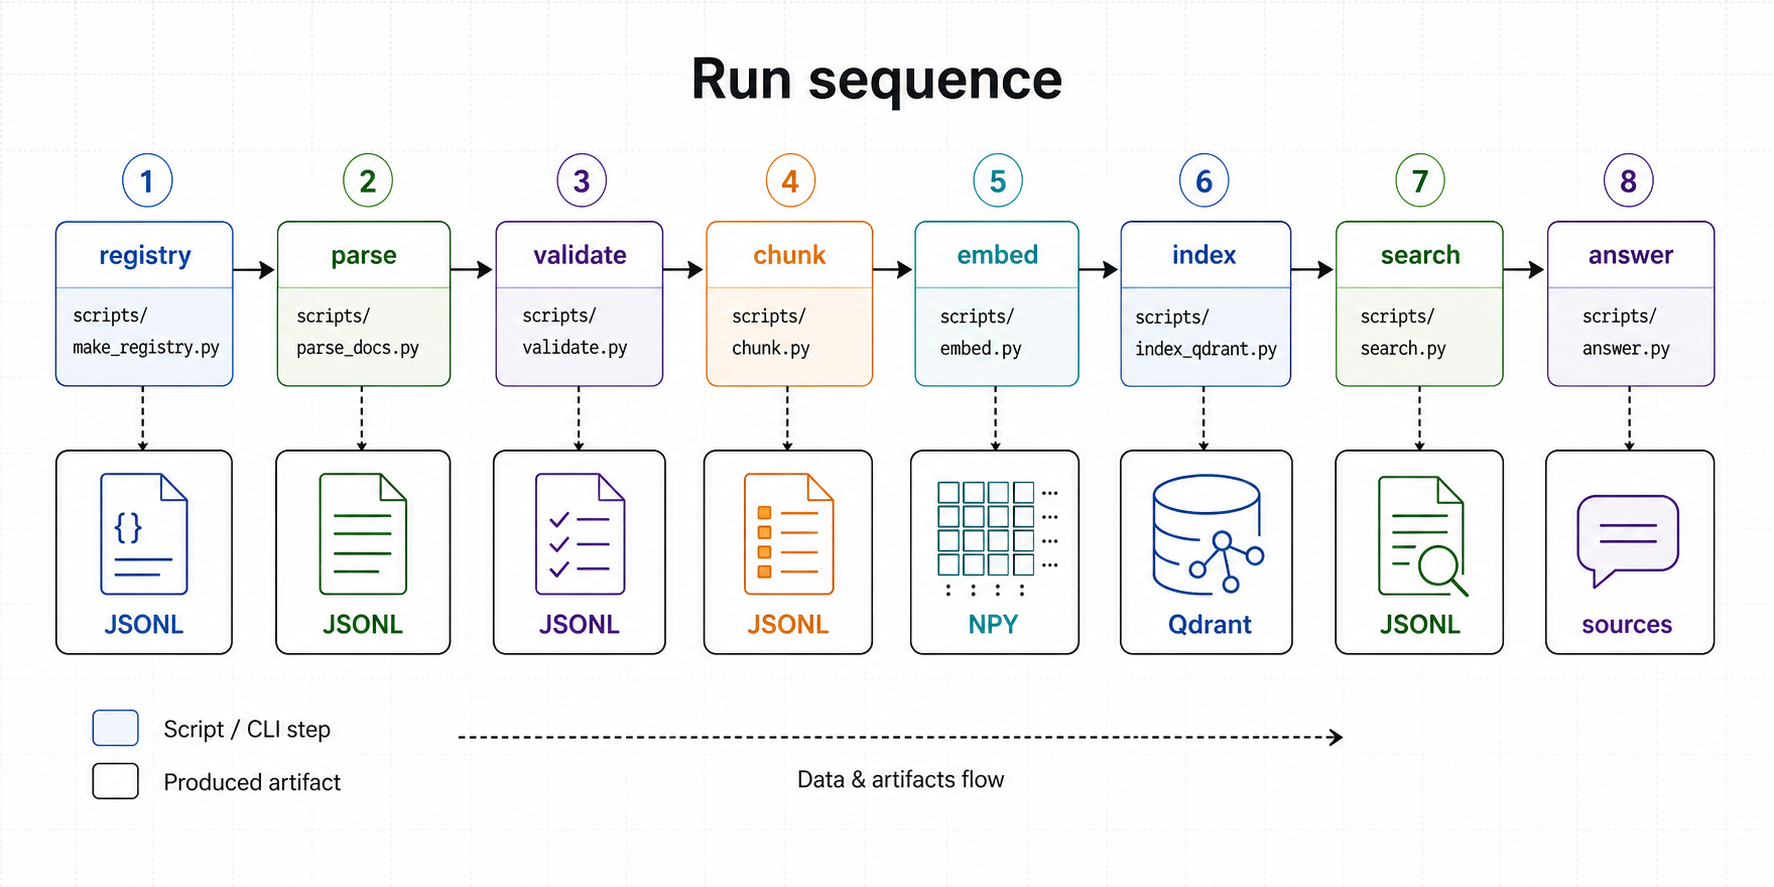
\includegraphics[width=\textwidth]{img/generated/rag_run_sequence.png}
\caption{Последовательность запуска базового MVP-пайплайна}
\label{fig:mvp-run-sequence}
\end{figure}

Рисунок~\ref{fig:mvp-run-sequence} показывает связь между CLI-этапами и создаваемыми артефактами. Такой порядок позволяет восстановить систему из исходных документов без ручного редактирования промежуточных файлов.

\section{Первичная проверка работоспособности}

Первичная проверка MVP проводилась на доменных вопросах по документам RobyMAX. Проверялось, что система возвращает релевантные чанки, формирует контекст и передает его LLM для генерации ответа на русском языке. При отсутствии сведений в найденном контексте система должна сообщать, что информации недостаточно, а не дополнять ответ внешними предположениями.

Для retrieval-части использовался набор \path{data/eval/retrieval_questions.jsonl}. По отчету \path{data/reports/eval_datasets_report.json} он содержит 150 вопросов: 45 технических, 45 продуктовых, 30 пресейл-вопросов, 15 сервисных и 15 коммерческих. Для каждого вопроса заданы релевантные \texttt{chunk\_id}, что позволяет автоматически проверить, попали ли ожидаемые фрагменты в top-k выдачи.

В качестве метрик использовались \texttt{Hit@K}, \texttt{MRR@K} и \texttt{Recall@K}. \texttt{Hit@K} показывает, найден ли хотя бы один релевантный фрагмент среди первых $K$ результатов. \texttt{MRR@K} учитывает позицию первого релевантного результата: чем выше релевантный чанк в выдаче, тем лучше значение. \texttt{Recall@K} отражает долю найденных релевантных фрагментов среди ожидаемых.

По отчету \path{data/reports/retrieval/retrieval_eval_report.json} для базового dense retrieval на 150 вопросах получены значения, приведенные в таблице~\ref{tbl:dense-metrics}.

\begin{table}[h]
\caption{Метрики базового dense retrieval для MVP}
\label{tbl:dense-metrics}
\centering
\begin{tabular}{|l|c|}
\hline
Метрика & Значение \\
\hline
Hit@1 & 0.4467 \\
Hit@3 & 0.6667 \\
Hit@5 & 0.7467 \\
MRR@5 & 0.5676 \\
Recall@5 & 0.6522 \\
\hline
\end{tabular}
\end{table}

Полученные значения подтверждают работоспособность базового dense-поиска, но не означают, что качество системы является окончательным. На данном этапе метрики используются как первичная инженерная проверка и точка отсчета для дальнейших итераций.

\section{Ограничения MVP}

Первая версия имеет ряд ограничений. Используется только базовый dense retrieval, поэтому система может пропускать фрагменты, где релевантность выражена точным термином, но embedding-модель не ставит такой фрагмент в top-k. Качество ответа зависит от качества найденных чанков, параметров context packing и prompt. В MVP не реализован полноценный диалоговый режим, отсутствует сложная проверка достаточности контекста, нет production API и пользовательского интерфейса. Оценка качества носит первичный характер и служит основой для последующих итераций.

\section{Выводы по главе}

В рамках практической части реализован базовый RAG-пайплайн: подготовка корпуса, парсинг, валидация, чанкинг, построение embeddings, индексация в Qdrant, dense retrieval и генерация ответа. Первичная проверка подтвердила работоспособность минимального сценария и позволила зафиксировать ограничения, которые должны быть устранены в следующих этапах работы.

%%% Local Variables:
%%% TeX-engine: xetex
%%% End:
